\section{Incorporating MINERvA components into ProtoDUNE-ND}
\label{sec:MINERvA}
The MINERvA experiment~\cite{minerva-nim} is located in the MINOS ND hall in which ProtoDUNE-ND will be installed, and is due to complete its data-taking in spring--summer 2019. The collaboration is currently considering its detector decommissioning plan, and it has been suggested that some components of the MINERvA tracking scintillator detector could be repurposed for ProtoDUNE-ND. As discussed in Section~\ref{sec:protodune-nd}, all DUNE ND designs considered in Ref.~\cite{dune_ndcsg} include some fast scintillator component. In this section, we outline the possible uses of the MINERvA detector components, and consider potential detector physics studies that they would bring to ProtoDUNE-ND.

\subsection{Repurposing the MINERvA detector}
The MINERvA detector is shown in Figure~\ref{fig:minerva_detector}. For the purpose of the discussion in this section, we will assume that the steel shield, scintillator veto plane, helium vessel, and nuclear targets region will be removed. 
\begin{figure}[htb]
  \centering
  \subfloat[Front view] {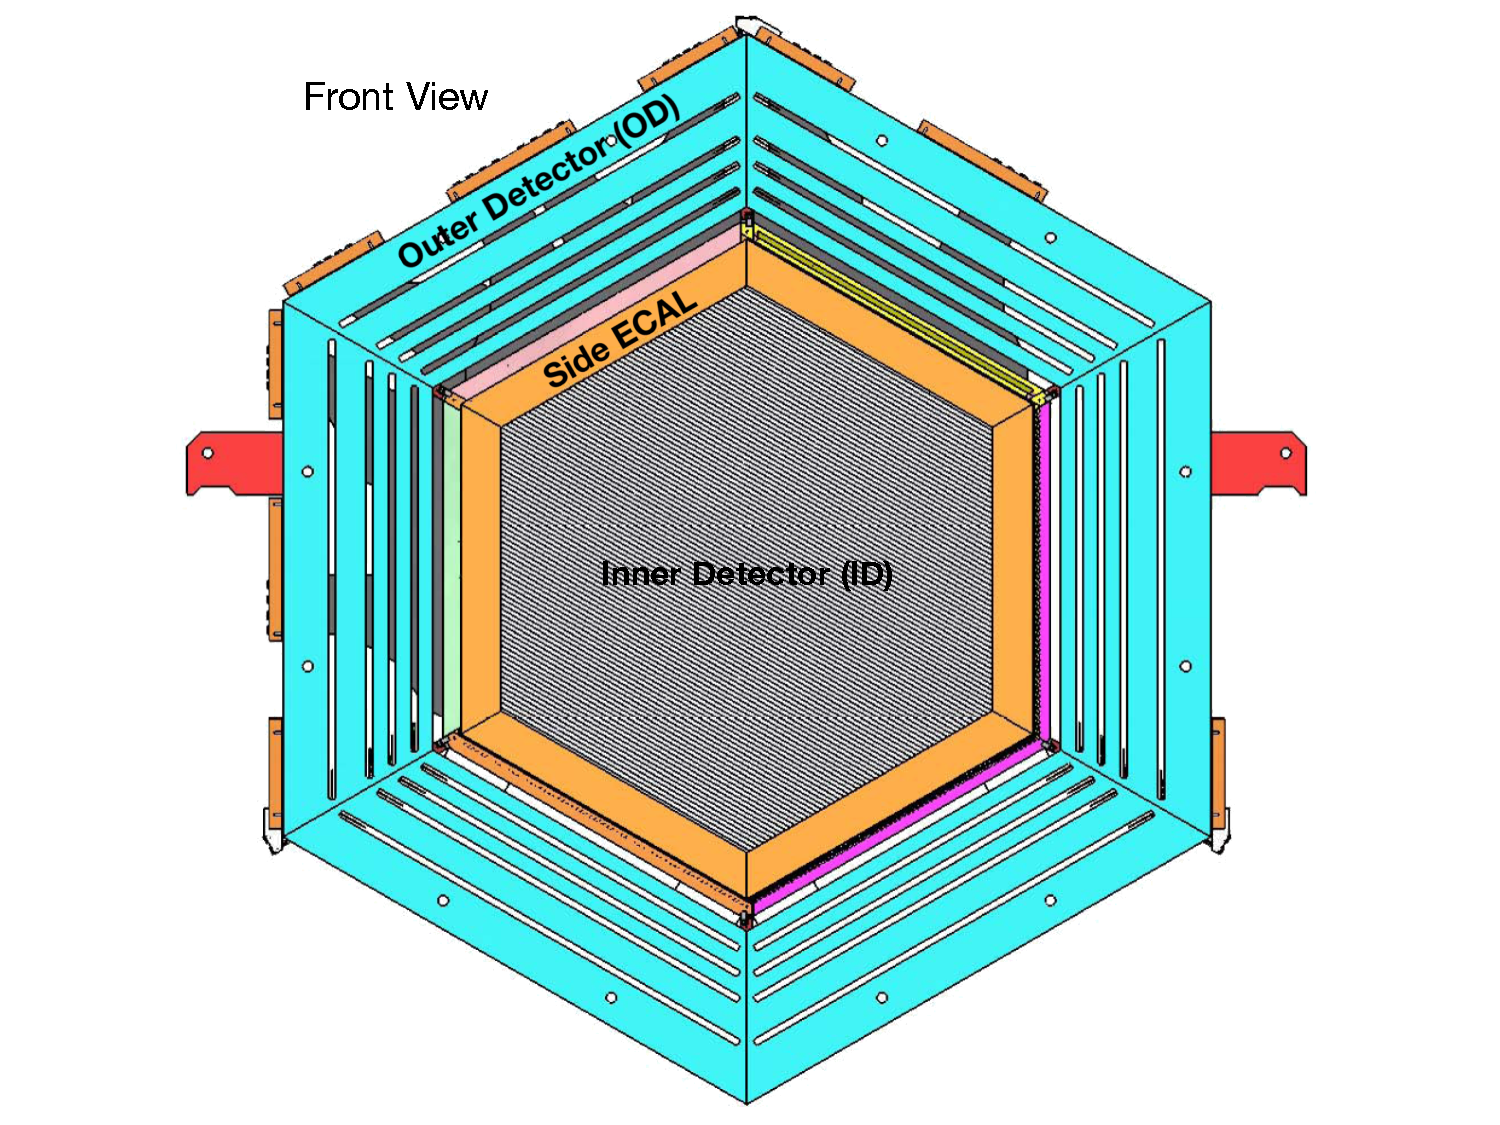
\includegraphics[width=0.35\textwidth]{plots/minerva_module_transverse.pdf}}
  \subfloat[Side view]  {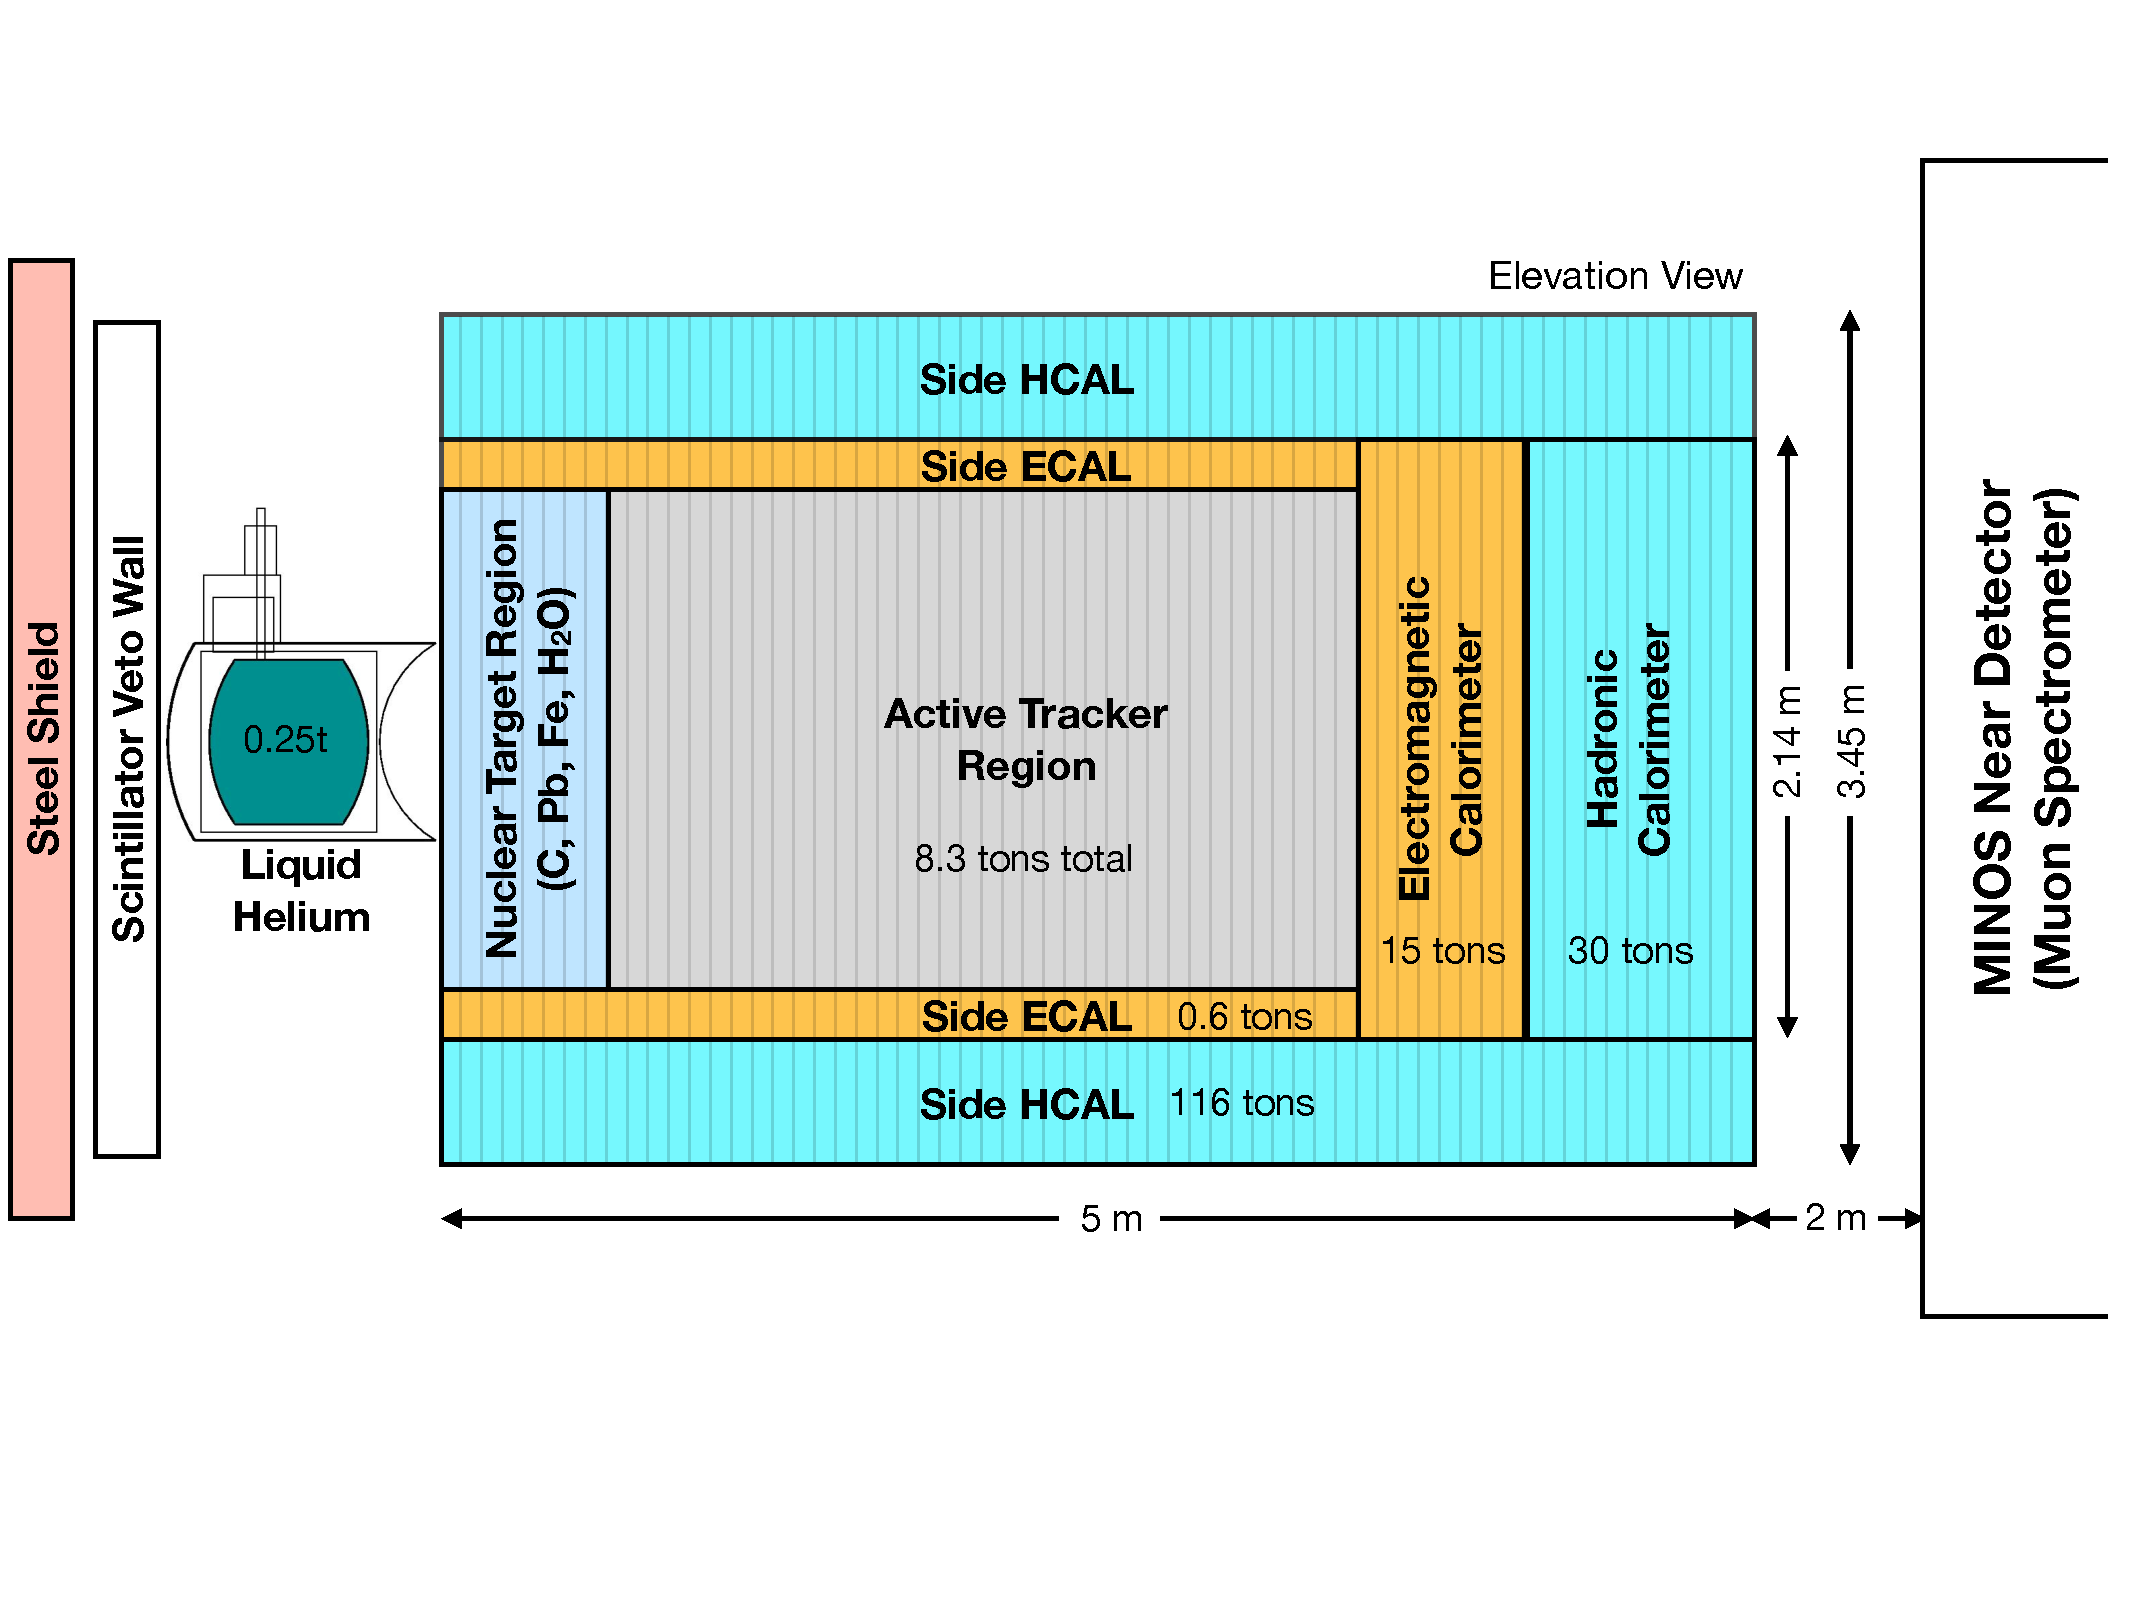
\includegraphics[width=0.60\textwidth]{plots/MINERvA_schematic.pdf}}
  \caption{Schematic of the MINERvA experiment. Reproduced from Figure 1 of Ref.~\cite{minerva-nim}.}
  \label{fig:minerva_detector}
\end{figure}

The remaining central tracking region, and both the electromagnetic and hadronic calorimeters are divided into modules which consist mostly of hexagonal scintillator planes, each made of 127 triangular scintillator bars, arranged in three different orientations (60$^\circ$ rotations between each plane). There are 62 modules in the fully-active tracker region, each composed of two scintillator layers. A 15 cm border of 0.2 mm thick lead on the downstream end of each module provides electromagetic calorimetry for particles exiting the side of the tracking region.

The downstream electromagnetic calorimeter is composed of 10 modules, each with two scintillator planes and a 0.2 mm thick lead plate on the downstream end. There are 20 modules in the downstream hadronic calorimeter, each with a single scintillator plane and a 2.54 cm thick hexagonal steel plane. The outer detector consists of a steel frame supporting structure with embedded scintillator planes, as can be seen in Figure~\ref{fig:minerva-module}, which turns the support structure into a hadronic calorimeter. The combination of the downstream and side electromagnetic and hadronic calorimeters allows for containment of most particles which escape from the central tracking region, and allows for particle identification and momentum measurements.

\begin{figure}[htb]
  \centering
  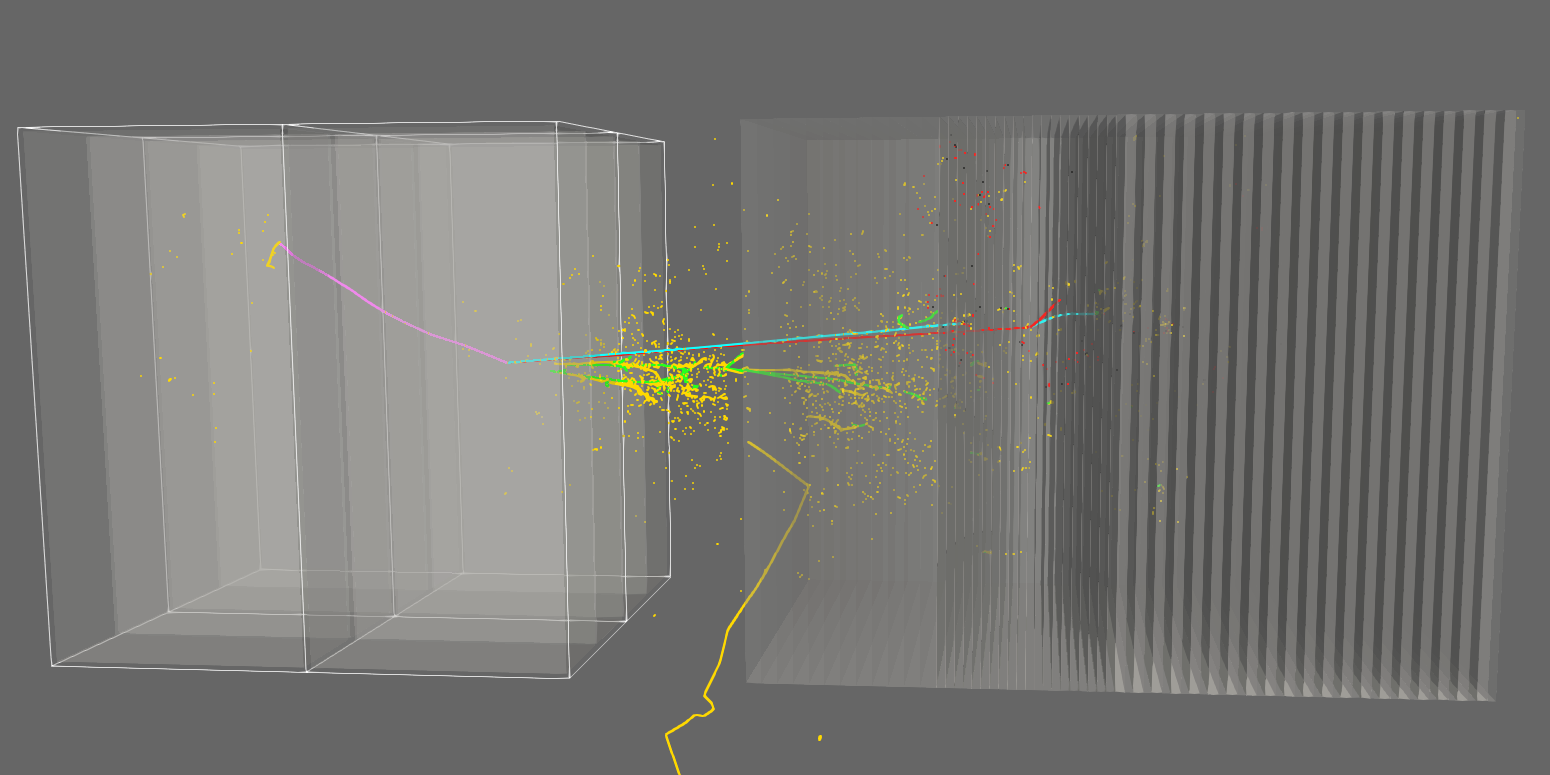
\includegraphics[width=0.8\textwidth]{{plots/Event_Displays_2x2_MINERvA/MINERvA_full_e70_rectangle_crop}.png}
  \caption{Example simulated event for a 7.0 GeV $\nu_{\mu}$--argon charged-current interaction, in which particles not contained in the ArgonCube 2x2 enter the MINERvA central tracking region downstream. Energy deposits are color-coded according to the particle type: $\pi^{\pm}$ --- blue; $\mu^{\pm}$ --- purple; $e^{+}$ --- green; $e^{-}$ --- yellow; proton --- red; recoiling nuclei --- black. The event vertex was randomly placed inside the active volume of the 2x2 Demonstrator module.}
  \label{fig:2x2+MINERvA_event}
\end{figure}
For the studies shown in this section, a simulation was performed approximating the downstream MINERvA central tracking region with a box of scintillator, and the ArgonCube 2x2 Demonstrator module upstream of the shortened MINERvA detector. \todo{Chris M to actually describe what this is...} An example event is shown in Figure~\ref{fig:2x2+MINERvA_event}, and can be compared with 2x2 only events in Figures~\ref{fig:argonbox_event_display} and~\ref{fig:leaky_event}. Note that this simulation only included the ArgonCube cryostat and MINERvA detector components, no material was included outside these (so escaping particles simply leave without ever re-interacting). This is unlike the previously described ArgonBox simulation, where a large box of argon was simulated (so escaping particles still re-interact). Events were again distributed uniformly throughout the ArgonCube active volume.

We note that the configuration discussed here may not be optimal. Some of the MINERvA scintillator modules could be used to provide vetos for particles entering or exiting the 2x2 cryostat, or to contain side-escaping showers. Indeed, the optimal design would also depend on whether use of the MINOS near detector as part of the ProtoDUNE-ND setup were supported. Here we discuss such possibilities in brief, and will wait to discover the viability of this project before embarking on more detailed studies.

\subsection{Detector physics studies possible with MINERvA components}
\todo{Add Patrick's plots here}

\subsubsection{Track matching}
\todo{Patrick needs to do this study!}

\subsubsection{Acceptance studies}
\todo{Update with higher statistics}

The inclusion of MINERvA in ProtoDUNE-ND will improve the acceptance of particles for various studies, some of which were described in Section~\ref{}. Here, we show how the efficiency for contained events compares for the 2x2+MINERvA setup desribed above, with MINERvA components located downstream of the ArgonCube 2x2 Demonstrator module, and for the 2x2-only case.
\begin{figure}[htb]
  \centering
  \subfloat[2x2-only]    {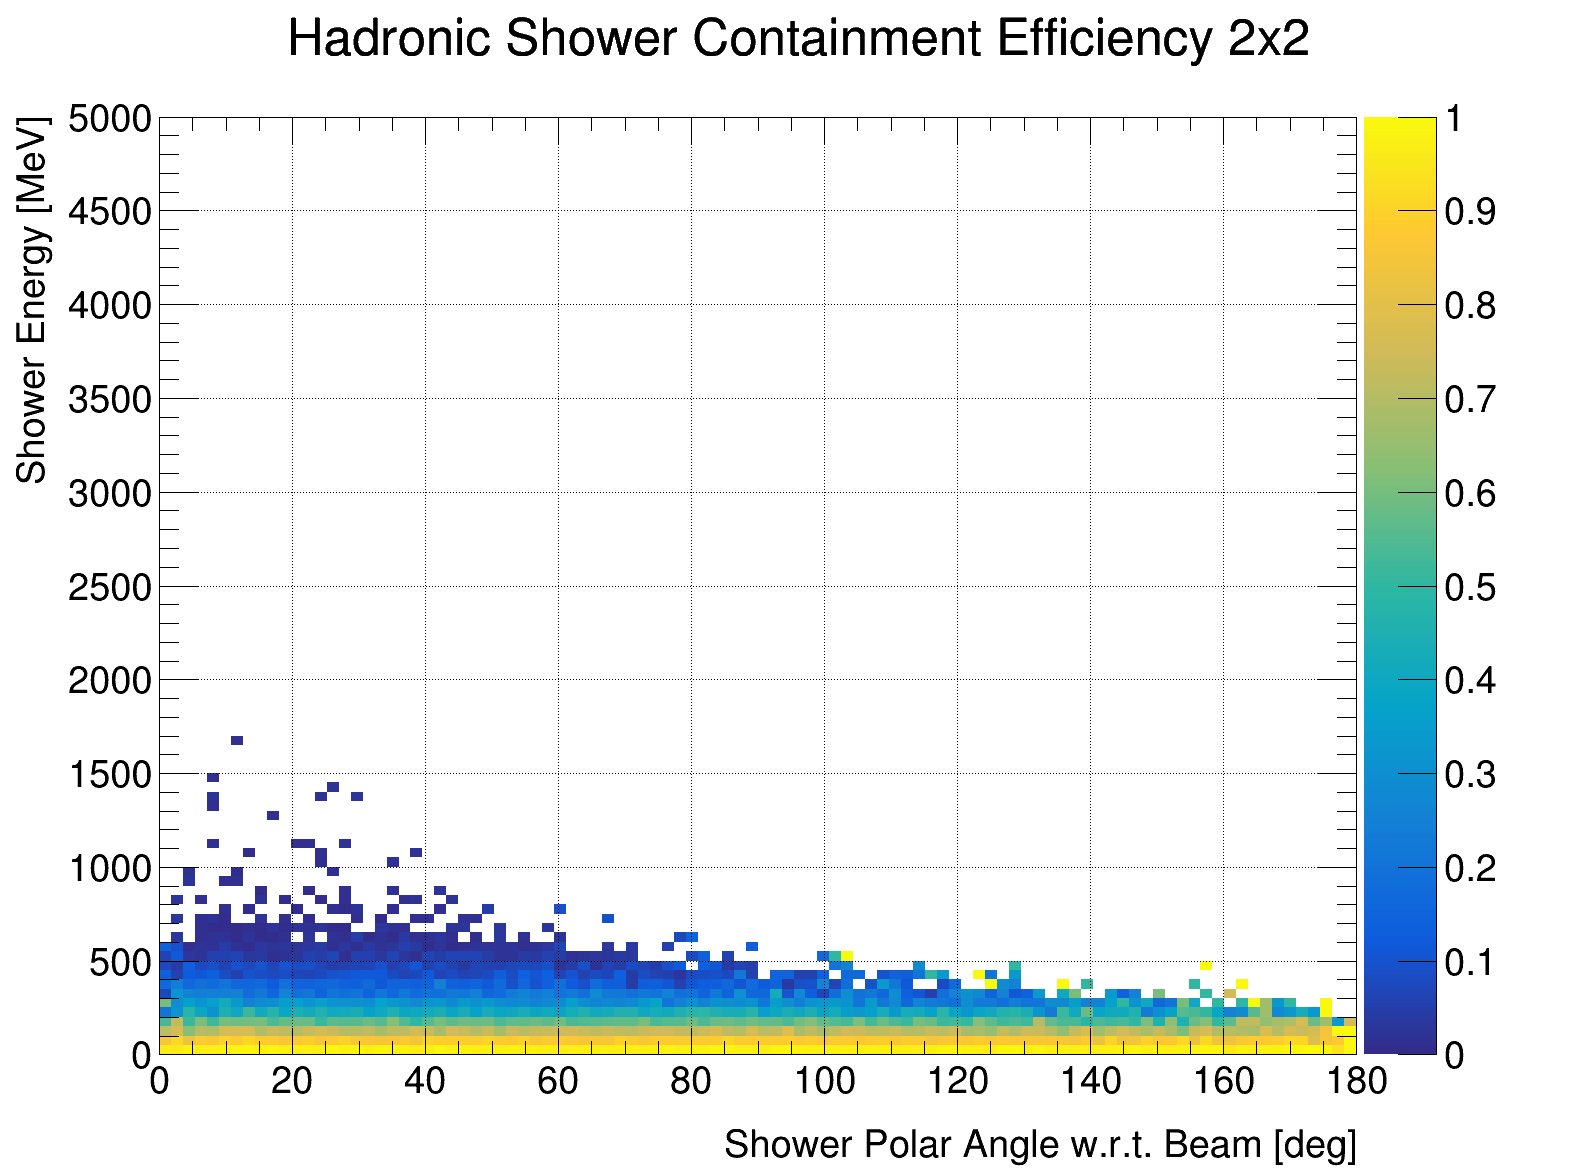
\includegraphics[width=0.45\textwidth]{plots/2x2_minerva_plots/H_cont_eff_2x2.png}}
  \subfloat[2x2+MINERvA] {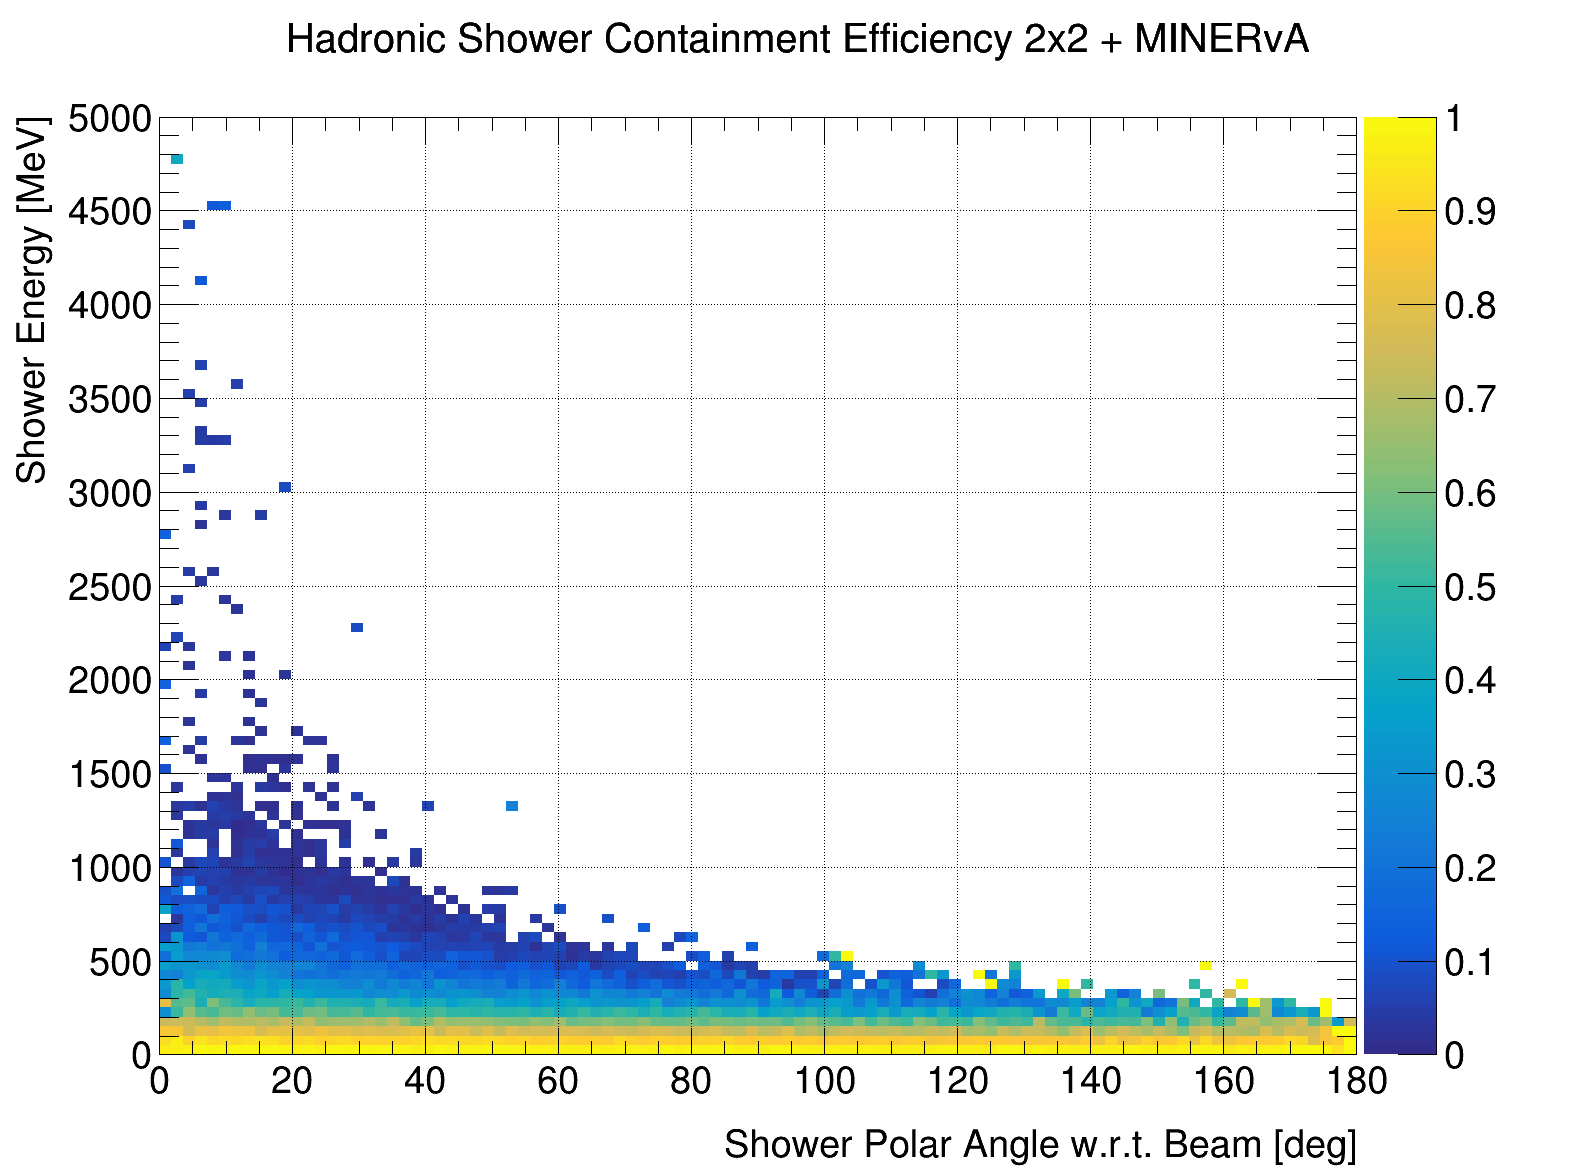
\includegraphics[width=0.45\textwidth]{plots/2x2_minerva_plots/H_cont_eff_2x2_MINERvA.png}}
  \caption{Schematic of the MINERvA experiment. Reproduced from Figure 1 of Ref.~\cite{minerva-nim}.}
  \label{fig:hadronic_containment}
\end{figure}

\begin{figure}[htb]
  \centering
  \subfloat[2x2-only]    {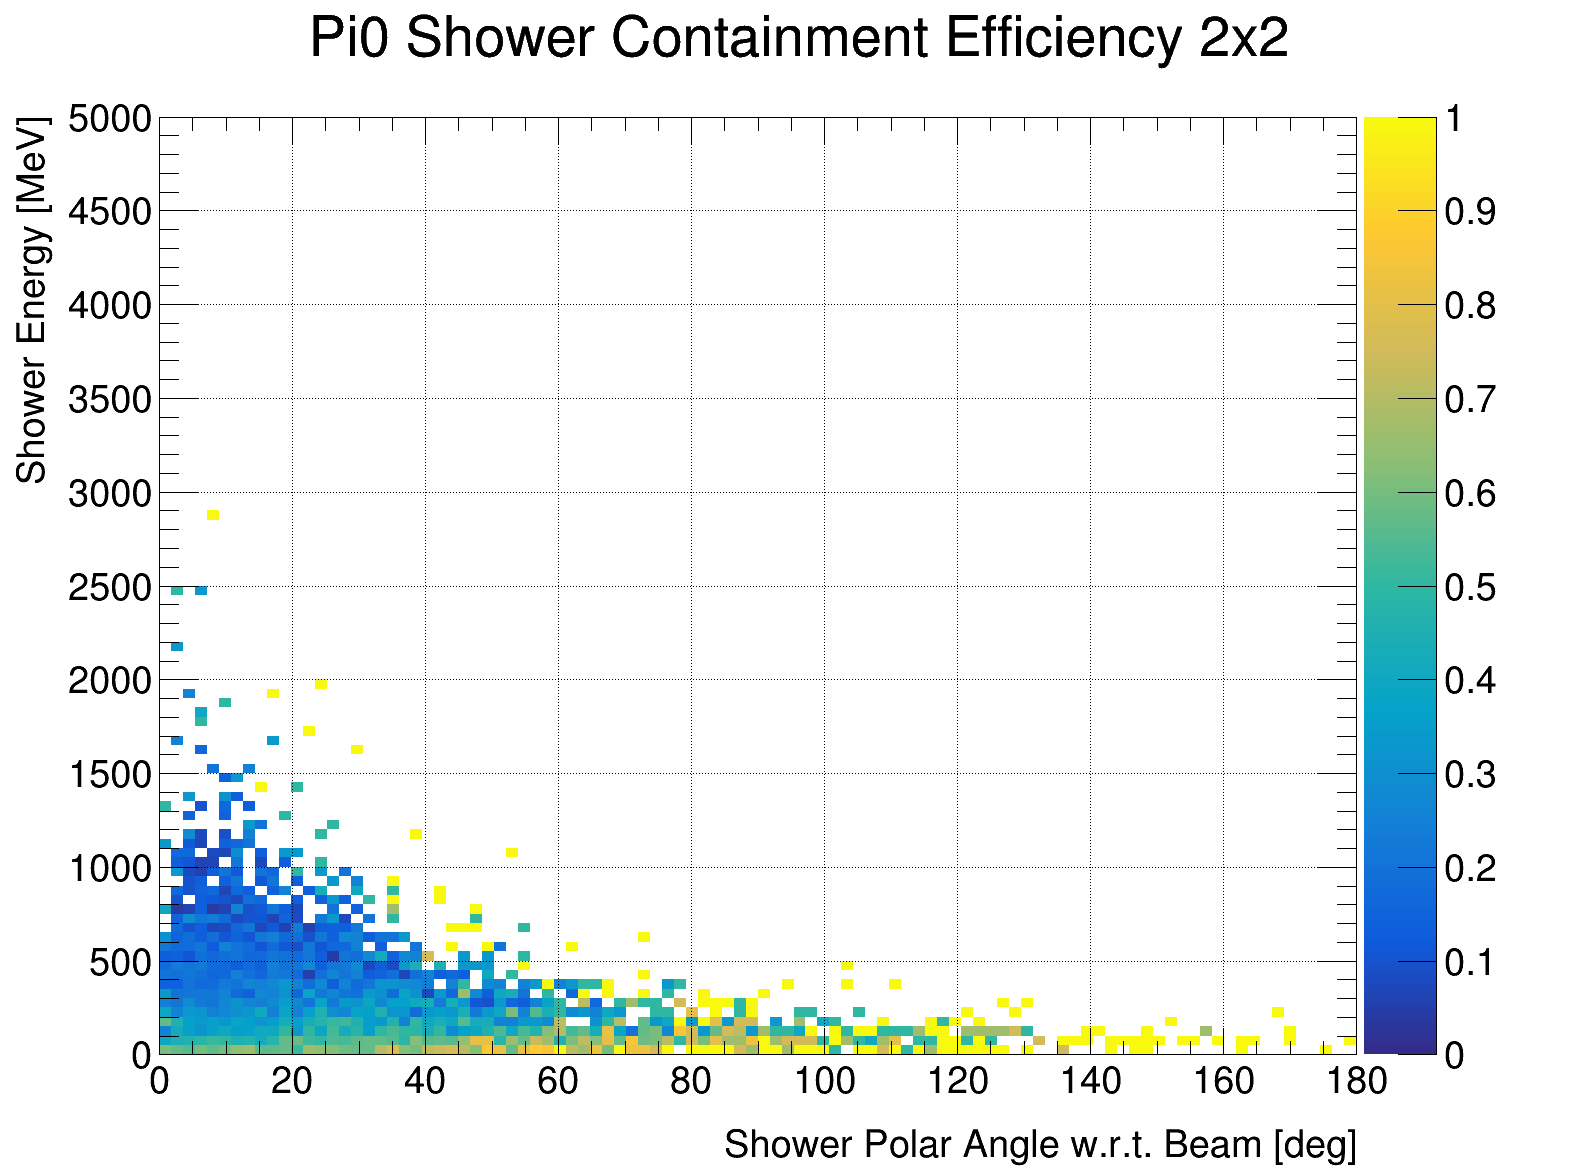
\includegraphics[width=0.45\textwidth]{plots/2x2_minerva_plots/Pi0_cont_eff_2x2.png}}
  \subfloat[2x2+MINERvA] {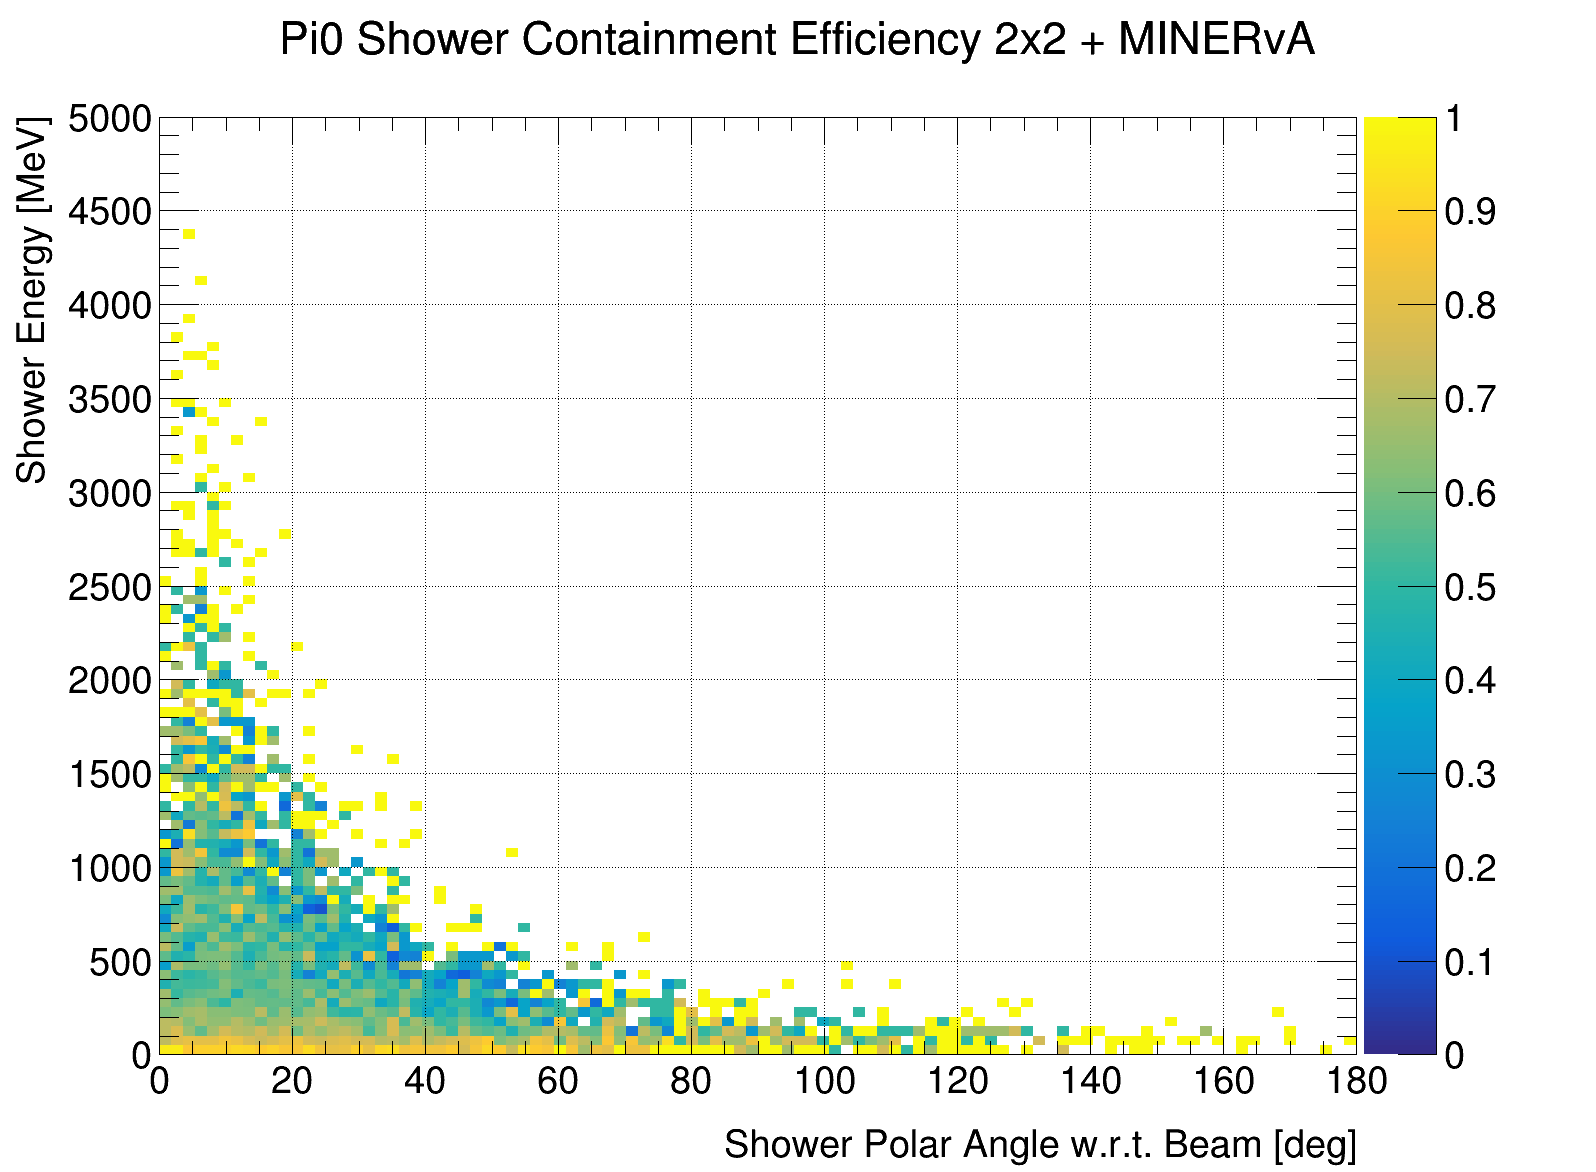
\includegraphics[width=0.45\textwidth]{plots/2x2_minerva_plots/Pi0_cont_eff_2x2_MINERvA.png}}
  \caption{Schematic of the MINERvA experiment. Reproduced from Figure 1 of Ref.~\cite{minerva-nim}.}
  \label{fig:pi0_containment}
\end{figure}

\subsubsection{Neutron tagging studies}

\subsection{Validation of multiple coulomb scattering}

\subsubsection{Use as a cosmic trigger}
\todo{Move some stuff from previous sections for this.}
